\documentclass[a4paper,11pt]{article}
\pdfoutput=1 % if your are submitting a pdflatex (i.e. if you have
             % images in pdf, png or jpg format)

\usepackage{jinstpub} % for details on the use of the package, please
                     % see the JINST-author-manual
%\usepackage{amsmath}
\usepackage{heppennames2}
\usepackage{hepnicenames}

%\usepackage{txfonts}
%\usepackage{newtxtext,newtxmath}
\usepackage{mathptmx}

%\usepackage[caption=false]{subfig}
\usepackage{subfloat}
%\usepackage{feynmp-auto}
\usepackage{color}
\unitlength = 1mm

%\makeatletter
%\def\endfmffile{%
%  \fmfcmd{\p@rcent\space the end.^^J%
%          end.^^J%
%          endinput;}%
%  \if@fmfio
%    \immediate\closeout\@outfmf
%  \fi
%  \ifnum\pdfshellescape=\@ne
%    \immediate\write18{mpost \thefmffile}%
%  \fi}
%\makeatother

\newcommand{\pt}{\ensuremath{p_{\mathrm T}}}

\newcommand{\mh}{\ensuremath{m_{H}} } 
\newcommand{\ptmiss}{\ensuremath{p_{\mathrm T}^{\mathrm{miss}}}}
\newcommand{\chisquare}{\ensuremath{\chi^2}}

\newcommand{\decayElectron}{\Pem\PAGne\PGnGt}
\newcommand{\decayMuon}{\PGmm\PAGnGm\PGnGt}
\newcommand{\decayPion}{\PGpm\PGnGt}
\newcommand{\decayRho}{\PGrP{\PGpm\PGpz}\PGnGt}
\newcommand{\decayAiPhoton}{\PaDoP{\PGpm\PGpz\PGpz}\PGnGt}
\newcommand{\decayAiPion}{\PaDoP{\PGpm\PGpm\PGpp}\PGnGt}
\newcommand{\decayThreePionPhoton}{\PGpm\PGpm\PGpp\PGpz\PGnGt}

\newcommand{\decayElectronShort}{\Pem\PAGne}
\newcommand{\decayMuonShort}{\PGmm\PAGnGm}
\newcommand{\decayPionShort}{\PGpm}
\newcommand{\decayRhoShort}{\PGrP{\PGpm\PGpz}}
\newcommand{\decayAiPhotonShort}{\PaDoP{\PGpm\PGpz\PGpz}}
\newcommand{\decayAiPionShort}{\PaDoP{\PGpm\PGpm\PGpp}}
\newcommand{\decayThreePionPhotonShort}{\PGpm\PGpm\PGpp\PGpz}

\newcommand{\rootS}{\ensuremath{\sqrt{s}} }


\title{\boldmath Reconstruction and classification of tau lepton decays at a future \Pem \Pep Linear Collider}


%% %simple case: 2 authors, same institution
%% \author{A. Uthor}
%% \author{and A. Nother Author}
%% \affiliation{Institution,\\Address, Country}

% more complex case: 4 authors, 3 institutions, 2 footnotes
\author[a,1]{B. Xu,\note{Corresponding author.}}
%\author[a,b,1]{F. Irst,\note{Corresponding author.}}
\author[a]{S. Green,}
\author[a]{J. S. Marshall,}
\author[a]{M. A. Thomson}
%\author[a,2]{T. Hird\note{Also at Some University.}}
%\author[c,2]{and Fourth}

% The "\note" macro will give a warning: "Ignoring empty anchor..."
% you can safely ignore it.

\affiliation[a]{Cavendish Laboratory,\\JJ Thomson Avenue, Cambridge, CB3 0HE, UK}
%\affiliation[b]{Another University,\\different-address, Country}
%\affiliation[c]{A School for Advanced Studies,\\some-location, Country}

% e-mail addresses: only for the forresponding author
\emailAdd{xu@hep.phy.cam.ac.uk}


\abstract
{
Seven tau lepton decay final states were studied using simulated data, for the proposed Compact Linear Collider. 
Tau leptonic physics is important. Its branching ratios measurements provide precision tests of the Standard Model. Spin state of a tau lepton can  be used to measure the CP properties of the Higgs boson, via the Higgs to a tau pair decay.
Classification efficiency of tau lepton decay is a benchmark of detector performance.
In this paper, seven final states were reconstructed and 




In this paper, the leptonic, hadronic 1-prong and hadronic 3-prong final sates of the tau lepton were classified for the centre of mass (\rootS) \Pem\Pep collision energies of 100, 200, 500 and 1000\,GeV and for the silicon-tungsten electromagnetic calorimeter (ECal) cell sizes from 3 to 20\,mm. The main challenge of the classification is the reconstruction and the separation of nearby photons as individual entities as well as he correct association of the tracks from the tracking system to the deposited energy shower. The unprecedented high classification rate of final decay separation is achieved. The overall hadronic decay selection efficiency is over 90\% for c.o.m. \rootS = 100\,GeV for the range of the ECal cell sizes, whilst the selection efficiency degrades significantly from 3\,mm to 20\,mm ECal cell size for \rootS = 500 and 1000\,GeV.
}
\keywords{TODO: Only keywords from JINST's keywords list please}


\arxivnumber{1234.56789} % only if you have one


% \collaboration{\includegraphics[height=17mm]{example-image}\\[6pt]
%   XXX collaboration}
% or
%\collaboration[c]{on behalf of XXX collaboration}


% if you write for a special issue this may be useful
\proceeding{N$^{\text{th}}$ Workshop on X\\
  when\\
  where}



\begin{document}
\maketitle
\flushbottom


\section{Introduction}

Tau lepton has been examined extensively in the past to study its physics and to use it as a detector benchmark test. 

Many experiments, including the Large Electron Positron Collider (LEP), has studied the tau lepton to great details \cite{Schael:2005am}. The total tau lepton hadronic decay width, which depends on the strong coupling constant, and the branch ratio of tau decay provide precision tests of the Standard Model and models beyond the Standard Model. The spin state of the tau lepton could be inferred from the kinematic properties of the decay products and can be used to measure the CP (the product of charge conjugation and parity symmetries) of the Higgs with a Higgs decaying to a tau pair channel. 

The efficiency of the final state separation of tau decay also provides a good benchmark of the detector performance. The tau lepton has a very short life time and it will decay before reaching the calorimeter. The typical decay products of the tau lepton are multiple photons and charged particles. The reconstruction of the multiple nearby photons requires an excellent electromagnetic calorimeter (ECal) resolution, whilst separating different charged particle relies on the performance of the tracking system. 


The study presented in this paper was done using the CLIC\_ILD detector concept with the PandoraPFA software package. A previous study with the International Large Detector (ILD) in the context of the International Linear Collider (ILC) was performed, where the impact of the varying the magnetic field and the size of the ECal were discussed. The CLIC\_ILD detector concept \cite{Linssen:2012hp} is designed for the Compact LInear Collider (CLIC) based on the ILD detector \cite{Abe:2010aa}, shown in figure~\ref{fig:ILD}, consisting of a vertex detector, tracking detectors, ECal, hadronic calorimeter (HCal) and a muon chamber. The ECal and HCal are optimised for the particle flow approach \cite{Thomson:2009rp} with high granularity in both longitudinal and transverse direction, providing unprecedented jet energy resolutions.

\begin{figure}[htbp]
\centering % \begin{center}/\end{center} takes some additional vertical space

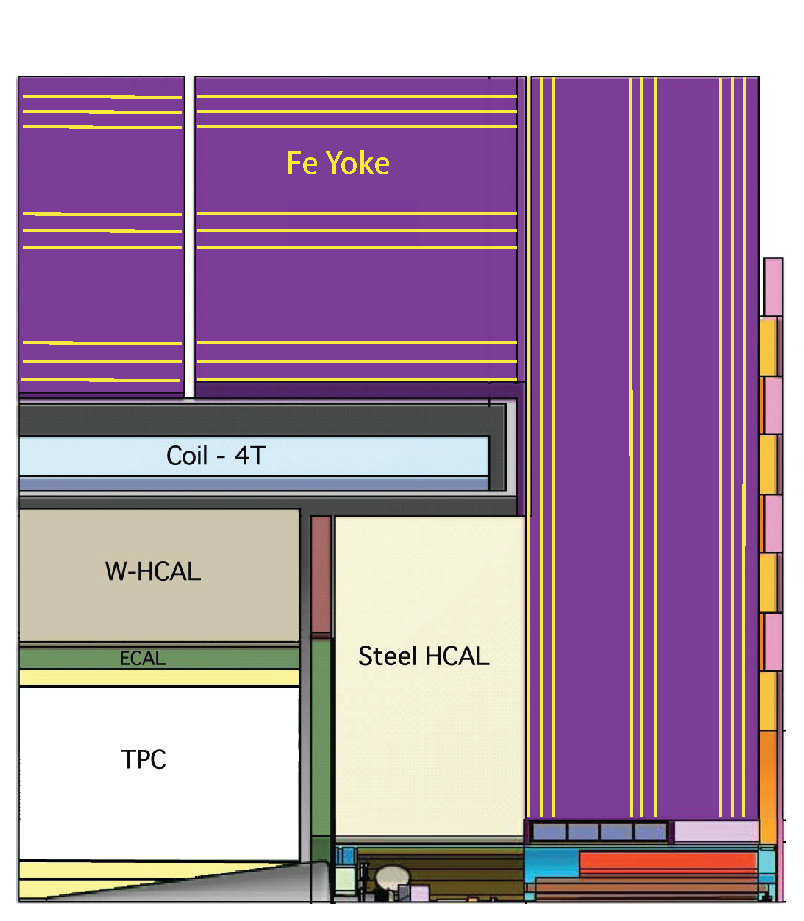
\includegraphics[width=.45\textwidth]{plots/CLICILD.eps}
\qquad
\caption{\label{fig:ILD} Longitudinal cross section of the top quadrant of CLIC\_ILD, taken from \cite{Linssen:2012hp}
}
\end{figure}


%Tau lepton has been studied in the Large Electron Positron Collider (LEP) and other experiments and the decay of the tau provides a probe to the precision test of the Standard Model. The spin of the tau lepton can also be inferred from the decay product and be used to measure the CP of the Higgs decaying to a tau pair.

%Tau lepton is important. Good to study. It has interesting physics, spins, differentiating higgs to z. 


%Final state separation of tau decay provides a good benchmark of the detector performance. The tau lepton has a very short life time and it will decay before reaching the calorimeter. As many of the final states of the tau decay consist of boosted charged particles with different numbers of photons and the ECal provides important calorimetric information for correctly reconstructing and separating nearby photons, this makes tau lepton decay final state separation suitable for the electromagnetic calorimeter (ECal) optimisation.

% The final sate separation is a good benchmark for the detector optimisation, as it tests the reconstruction of nearby photons, electron and muons. 


%A previous study with the International Large Detector (ILD) in the context of the International Linear Collider (ILC) was performed \cite{Tran2016}. Photons were reconstructed with GARLIC software package \cite{Reinhard2009,Jeans:2012jj} where the impact of the varying the magnetic field and the size of the ECal were discussed. It was shown that about 95\,\% \Ppiminus\Pnut and 90\,\% \Prhominus\Pnut and \Pai\Pnut final states were correctly reconstructed.

%It was shown that the ILD could separate the one \Ppipm hadronic decay final states with high probabilities.

% Previous study has been done on the ILD detector. Results were shown. Impact on B field and ECal sizes were studied.

% A new CLIC detector model is being designed with a Silicon tracking system in mind.

%Studied was done on CLIC\_ILD detector. CLIC\_ILD is designed based on the ILD detector, with a complicated tracking system including a TPC, a Si W fine granular ECAL aimed for PFA. A new CLIC detector model is being designed with a Si tracking system in mind.

The difficulty of the \PGt decay mode separation is to correctly reconstruct photons in the final states. Two main features of the reconstruction software, PandoraPFA \cite{Marshall:2015rfa}, help to separate the final states. Firstly, the iterative track cluster association algorithms connecting reconstructed tracks to the cluster showers in the calorimeters, providing a good identification of the charged particles and leave a cleaner environment for the neutral particles. Secondly, a transverse calorimeter shower profile based photon reconstruction algorithm carefully identifies and separates nearby photons, using a likelihood photon identification algorithm. Along side with other reconstruction algorithms in the PandoraPFA software, charged particles and photons are well reconstructed and used as inputs for \PGt decay mode separation.

In this paper, we present a study for the separation of tau lepton decay final states, to demonstrate the high classification rate, with varying sizes of the ECal cells and the centre of mass  energies (\rootS) of the \Pem\Pep $\to$ \PGtm\PGtp interaction.


\section{Simulation and Reconstruction}

Simulated Monte Carlo (MC) samples were generated with the generator software WHIZARD 1.95 \cite{whizard}, where PYTHIA 6.4 \cite{Sjostrand:1995iq} is used for the hadronisation and is tuned to the LEP results \cite{}. TAUOLA \cite{Jadach:1993hs} is used to describe the \PGt lepton decays with correct spin effect. The initial state radiation (ISR) and the beam induced background were not simulated, but final state radiation (FSR) was simulated. 

Around two millions MC events per ECal cell size and per \rootS energy were simulated. An event was considered if the event passes a set of cuts at generator level, listed here
\begin{itemize}
  \item the final state photons not converting to electron pair in the tracker,
  \item the tau leptons decaying in the barrel and the end cap regions, which are defined as polar angle between 0.3 to 0.6 rad and 0.8 to 1.57 rad, and
  \item the visible energy of the tau lepton decay products more than 5\,GeV, where the visible energy of the tau lepton decay is defined as the energy of the tau minus the energy of the tau neutrino. 
\end{itemize}

Events were simulated with software MOKKA \cite{MoradeFreitas:2002kj} with the CLIC\_ILD detector geometry description, based on the GEANT 4 package  \cite{Agostinelli:2002hh}. Events were reconstructed with ilcsoft version v01-17-07 \cite{Gaede:82475} and PandoraPFA version v02-02-00 \cite{Marshall:2015rfa}, where the photon reconstruction is described in \cite{Xu:2016rcz}.

The events were simulated at \rootS = 100, 200, 500 and 1000 GeV, with different ECal square cell sizes of 3, 5, 7, 10, 15 and 20 mm.

\section{Analysis strategy}

\begin{table}[htbp]
\centering
\caption{\label{tab:decay_mode} Branching fractions of the seven \PGtm decays in this study, taken from \cite{Agashe:2014kda}. \PGtp decays similarly to \PGtm.}
\smallskip
\begin{tabular}{|l |r|}
\hline
  \textbf{Decay mode} & \textbf{Branching fraction / \%} \\
\hline
  \decayElectron        & 17.83$\pm$0.04   \\
  \decayMuon  	& 17.41$\pm$0.04  \\
  \decayPion     	& 10.83$\pm$0.06   \\
  \decayRho	& 25.52$\pm$0.09 \\
  \decayAiPhoton	& 9.30$\pm$0.11    \\
  \decayAiPion  	    & 8.99$\pm$0.06  \\
  \decayThreePionPhoton  	    & 2.70$\pm$0.08  \\

\hline
\end{tabular}
\end{table}

Seven decay final states of the tau lepton shown in table~\ref{tab:decay_mode} were studied, covering 92.58\,\% of all tau decays. The decay modes not covered have branching fractions lower than 1\% each. These final states can be classified into three categories: leptonic decays, one-prong with photons and three-prong with photons. 

The channel \Pem\Pep $\to$ \PGtm\PGtp contains two \PGt travelling back-to-back. As we are interested in single \PGt decay, the detector fiducial space is divided into two halves, each corresponding to one \PGt. The division was performed with the thrust axis, where defined as 
$T = max_{\hat{n}} \frac {\sum_i \left| p_i . \hat{n} \right|}{\sum_i \left| p_i \right|}$. $p_i$ is the momentum three-vector of a Particle Flow Object (PFO), $\hat{n}$ is the thrust axis, a unit 3-vector that maximise the thrust, $T$. PFOs were separated into two collections based on the sign of the dot product between the momentum and the thrust axis vector.

\begin{figure}[htbp]
\centering % \begin{center}/\end{center} takes some additional vertical space

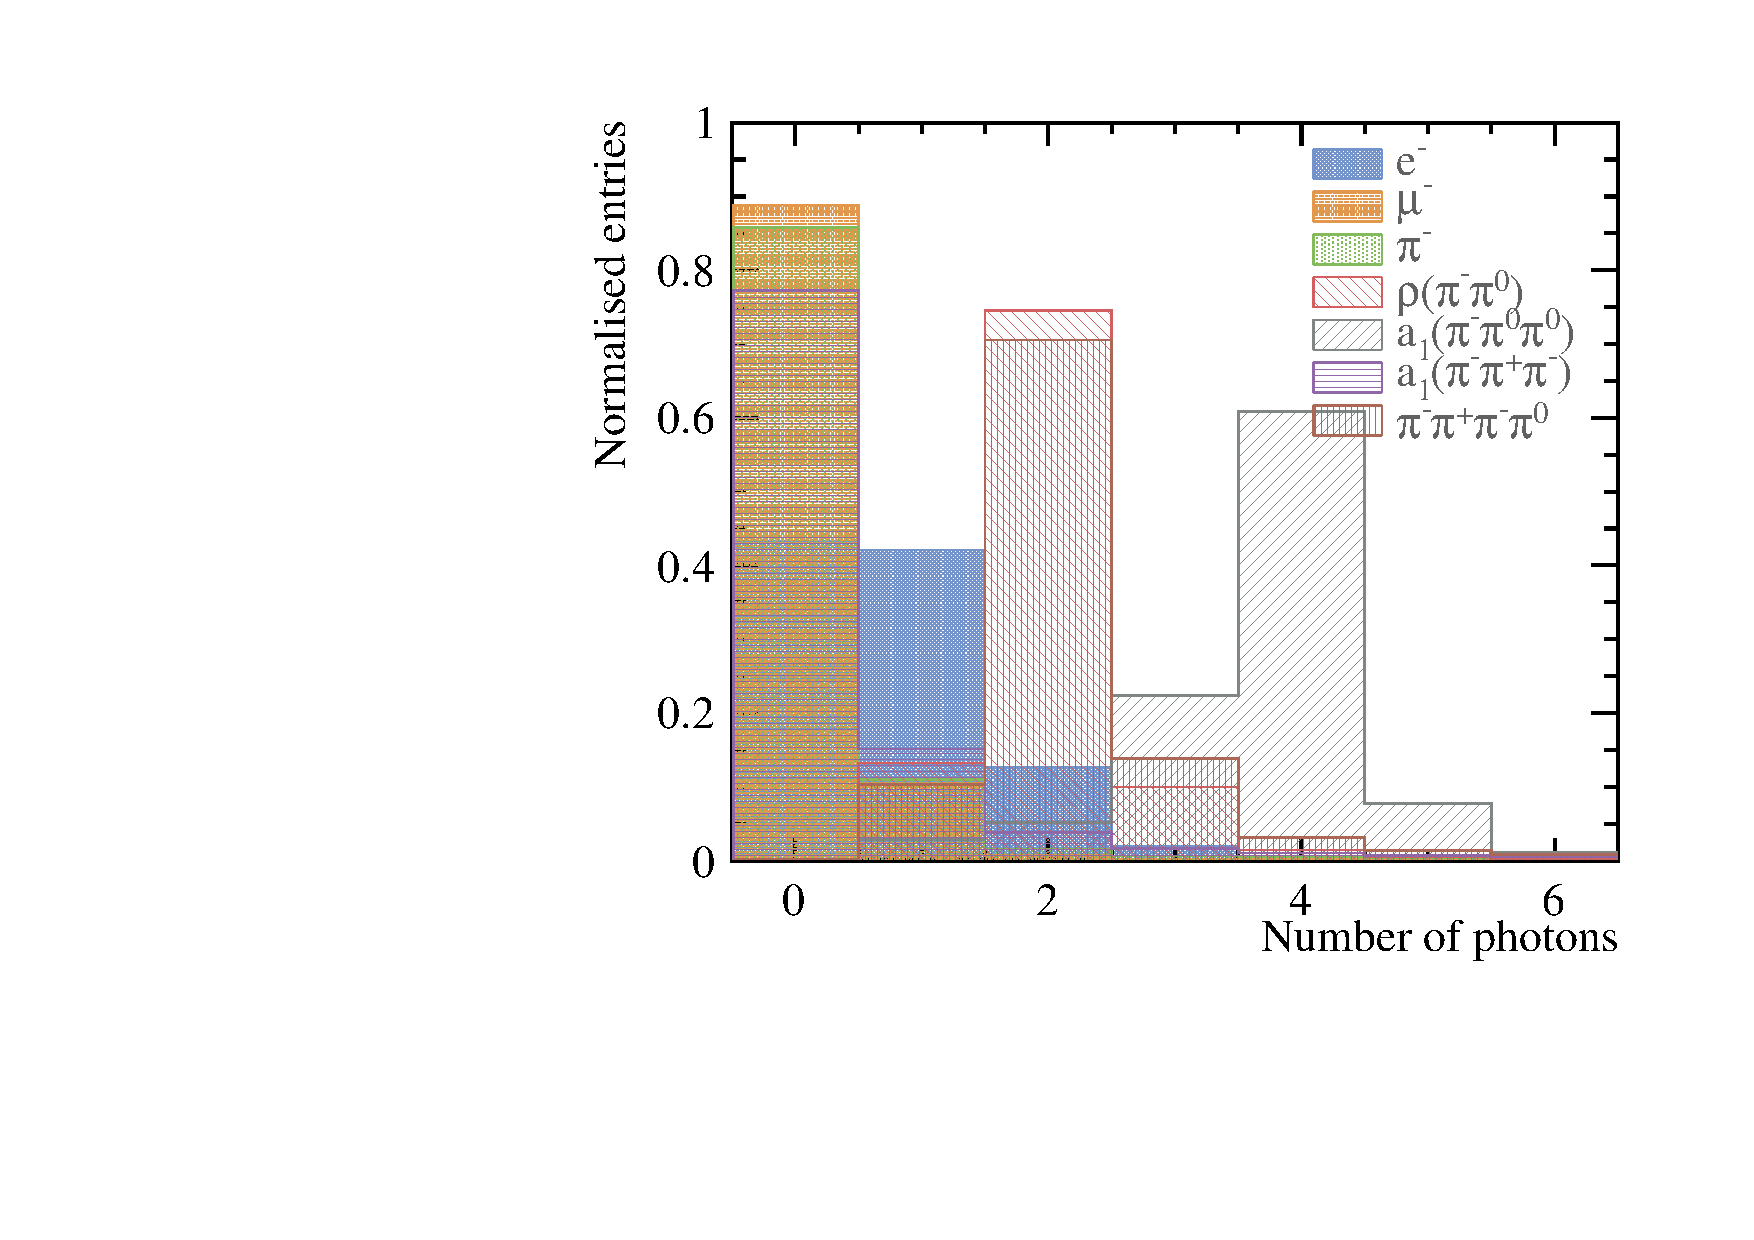
\includegraphics[width=.45\textwidth]{plots/var/nPhoton_100GeV_improved} 
\qquad
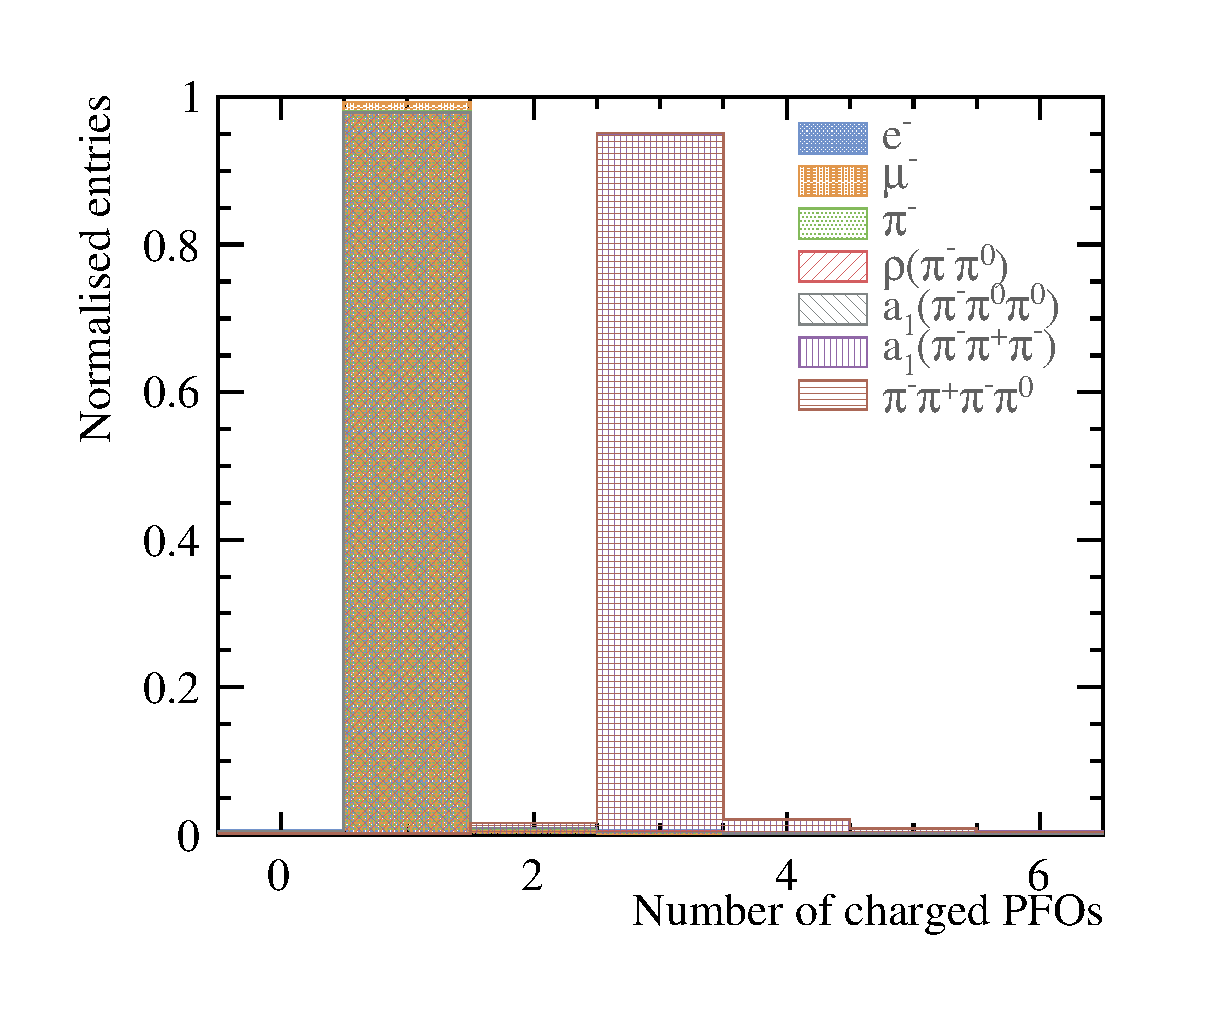
\includegraphics[width=.45\textwidth]{plots/var/nCharge_100GeV_improved} 
\qquad
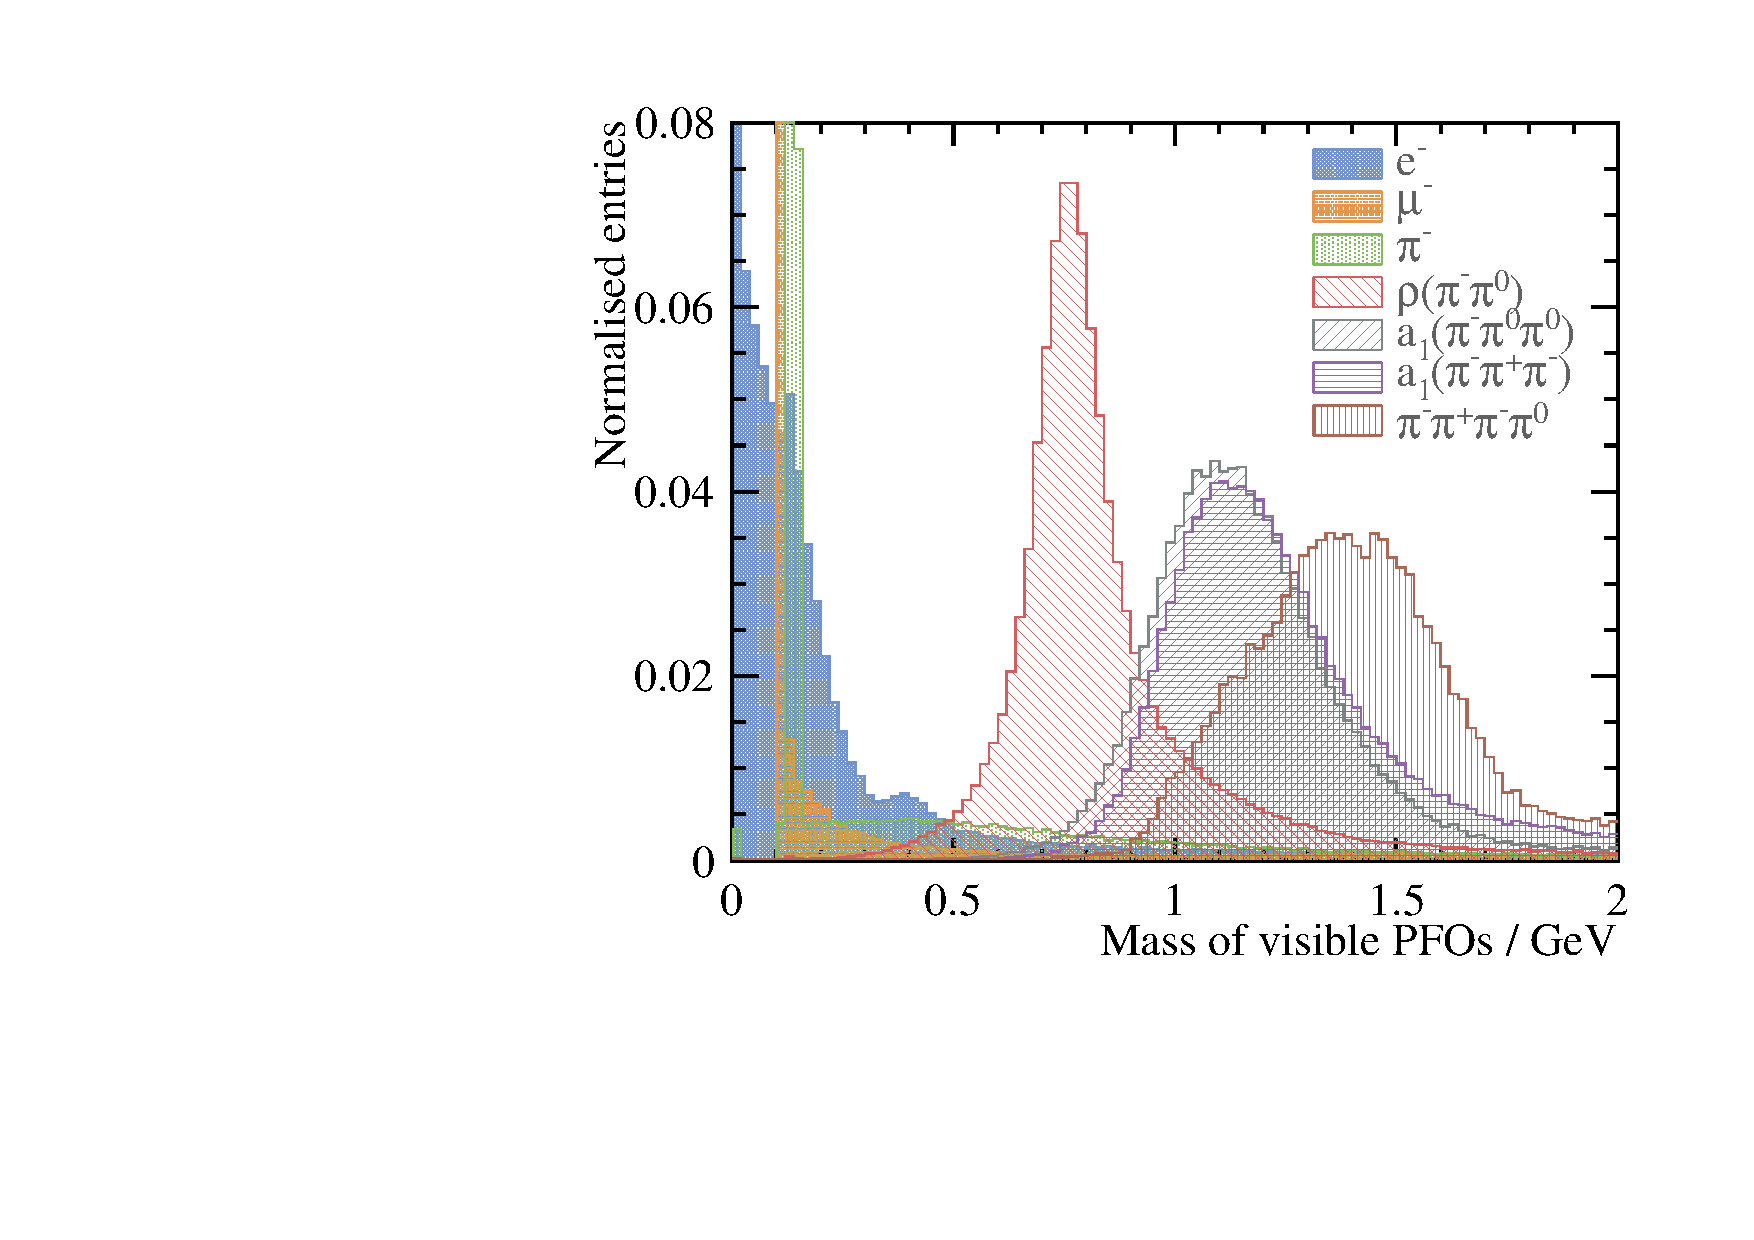
\includegraphics[width=.45\textwidth]{plots/var/mVis_100GeV_improved_zoom}
\qquad
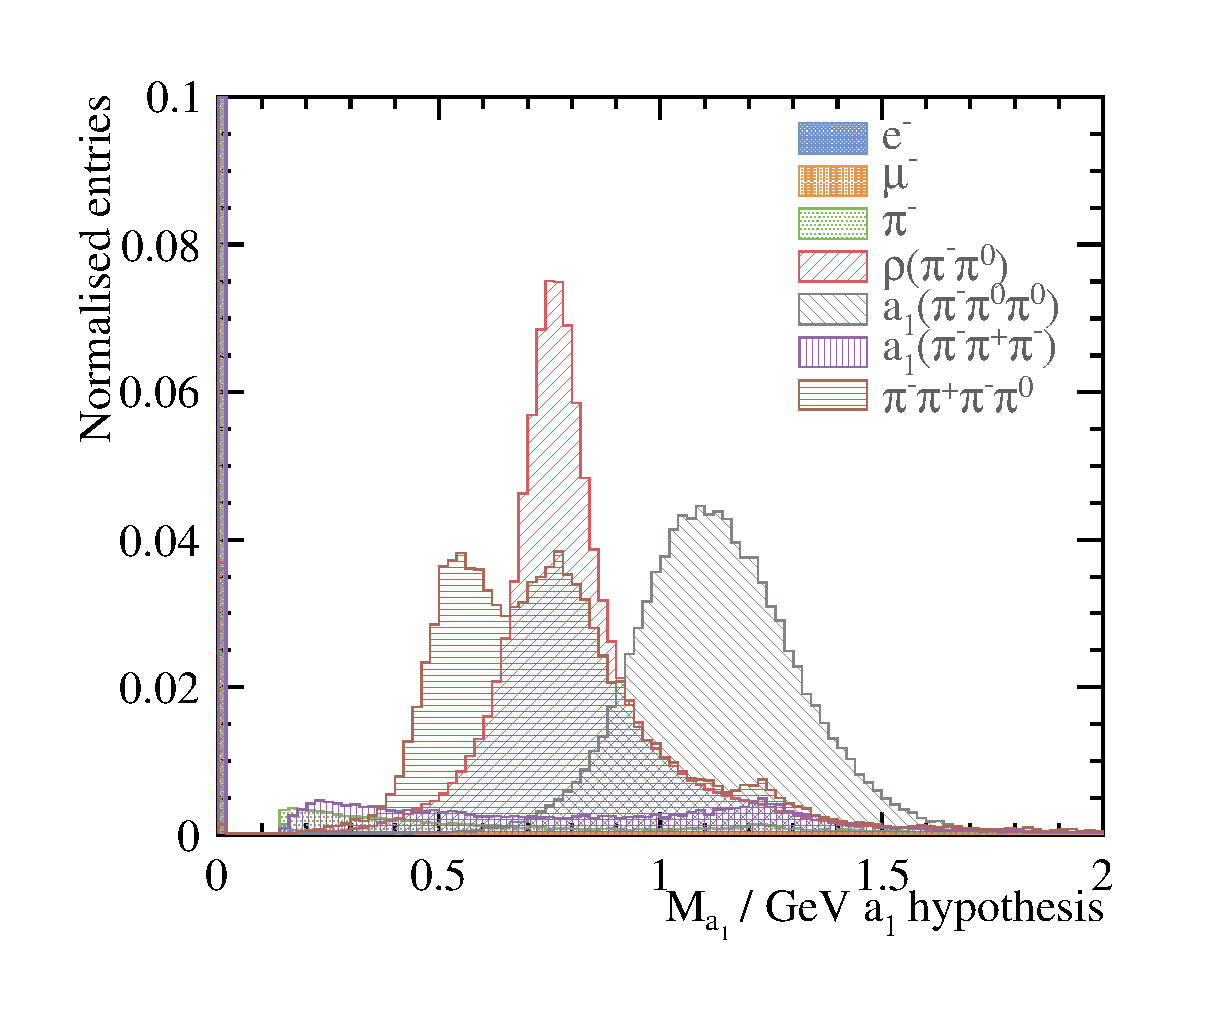
\includegraphics[width=.45\textwidth]{plots/var/mA1A1Fit_100GeV_improved_zoom}
\qquad

\caption{\label{fig:nPfos} 
The example normalised distribution for discriminative variables for seven final states, \decayElectron, \decayMuon, \decayPion, \decayRho, \decayAiPhoton, \decayAiPion and \decayThreePionPhoton, separated with truth information,  with \rootS = 100 \,GeV for nominal CLIC\_ILD detector model. The top left and top right, bottom left and bottom right plots are the normalised entries against the number of photons, number of charged PFOs, invariant mass of visible PFOs and the invariant mass of \decayAiPhotonShort for \decayAiPhotonShort hypothesis, respectively. There is a clear distinction between different final states in each plot.
}
\end{figure}

To identify the decay mode of \PGt from the decay products, a set of discriminative variables were carefully calculated and chosen. The full list of variables can be found in the appendix. There are 29 variables used in the multivariate analysis. The reason for the large number of variables is due to training seven decay modes at once, which will be discussed later.

Some of the variables with most discriminative power are shown in figure~\ref{fig:nPfos}. 

Number of photons is an important variable for separating decay modes. This information is only available due to the excellent photon reconstruction. Shown in figure~\ref{fig:nPfos}, the majority of \decayMuon, \decayPion and \decayAiPion final states have zero photon reconstructed. The \decayElectron final state event have one photon reconstructed instead of zero, due to the FSR effect. \decayRho and \decayThreePionPhoton have nearly 80\% events with two reconstructed photons, whilst \decayAiPion have over 60\% events with four reconstructed photons. The loss is efficiency is due to the increasing difficulty to separate nearby photons.

The number of charged PFOs can clearly separate the leptonic and 1-prong final states, from the 3-prong final states, shown in figure~\ref{fig:nPfos}. The efficiency of leptonic final states are over 98\%. 

The invariant mass of the visible PFOs shows clear differences between different final states. \decayRho, \decayAiPhoton and \decayAiPion distribution show clear resonance at \PGrP and \Pa. \decayElectron, \decayMuon and \decayPion distribution show much smaller invariant mass and \decayThreePionPhoton shows a large invariant mass than \Pa. The \decayElectron final state has a long tail of invariant mass due to the extra photons from the FSR.

For the final states with resonance, additional $\chi^{2}$ minimisation test for particle pairings have been performed. For example, \decayAiPhoton final state, the  $\chi_{\Pa}^{2}$ to minimise is,

\begin{equation}
\label{eq:a1}
\chi_{\Pa}^{2} = {\left(\frac{m_{\Pa,fit} -  m_{\Pa}}{\sigma_{\Pa}}\right)}^{2} + {\left(\frac{{m_{\PGpz,fit}} -  m_{\PGpz}}{\sigma_{\PGpz}}\right)}^{2} + {\left(\frac{{m_{\PGpz^*,fit}} -  m_{\PGpz}}{\sigma_{\PGpz}}\right)}^{2}  \,,
\end{equation}

where $m_{\PGpz,fit}$ and $m_{\PGpz^*,fit}$  are the invariant masses of all possible two photons combinations, $\sigma_{\Pa}$ and $\sigma_{\PGpz}$ are the half width of the invariant mass distribution of reconstructed \Pa and \PGpz using the truth information, and $m_{\Pa}$ and $m_{\PGp}$ are the masses of \Pa and \PGpz, taken from \cite{Agashe:2014kda}. If there are two or three photons, the $\chi_{\Pa}^{2}$ expression will be reduced and not including $m_{\PGpz^*,fit}$ term. If there are fewer than two photons, the $\chi_{\Pa}^{2}$ expression would only contain $m_{\Pa,fit}$ term.


For the \decayRho final state, a similar $\chi_{\PGr}^{2}$ test for \PGr hypothesis is used to extract $m_{\PGr,fit}$ and $m_{\PGpz,fit}$ variables. $\chi_{\PGr}^{2}$ is similar to $\chi_{\Pa}^{2}$ with \PGr replacing \Pa and only one $m_{\PGpz,fit}$ term.


Figure~\ref{fig:nPfos} shows the $m_{\Pa,fit}$ where \decayRho, \decayAiPhoton  and \decayThreePionPhoton final states contribute to the \Pa resonance, although only \decayAiPhoton final has a real \Pa resonance. This is due to the structure of the  $\chi_{\Pa}^{2}$ minimisation function allowing final states with more than two photons and one \PGppm to contribute.

Additional variables are calculated using the calorimeter information, the comparison with the electromagnetic shower profile, the matching between the track and the cluster, the energy and invariant masses for different types of particles. Extra variables regarding to the electromagnetic shower profile are used to distinguish electrons from charged pions.

%, listed in Table XX. Note that XX variables were specialised in separating a electron from a pion. XX variables were made to test the hypothesis of XX particles. The rho hypothesis is to find the best rho decay candidates by minimising chi squared according to $aa$, where X is all possible charge pions, Y is all possible 2 photons. The formula will reduce accordingly if there is 1 photon. Similarly, the a1 decaying to 1 pion 4 photon hypothesis is done in a same fashion with Chi squared function XX, , where X is all possible charge pions, Y is all possible 2 photons. The formula will reduce accordingly if there are 2 or 3 photons.

Energy of the \PGt is assume to be the same as the energy of \Pepm beam, which is half of the \rootS energy. Recoil momenta were calculated assuming the \Pem\Pep collision happened at the centre of mass energy. Both assumptions are largely valid when there is no ISR contribution. %The variables of energy ratios instead of the raw energies were calculated to make the MVA process more generic across different c.o.m. energies.

For the multivariate analysis, the multiclass class of the TMVA package \cite{Therhaag:2009dp} was used to perform a multiclass classification, which trains the seven final states simultaneously. The multiclass class is an extension of the standard two-class signal-background classifier. For each final state, the multiclass classifier will train the final state as the signal against all other final states as the background. This process is repeated for each final state. The classifier output for a single event is a normalised response for each final state, where the sum is one. The response of each final state of a event can be treated as the likelihood. The event is classified into a particular final state if the final state has the highest classifier output response. The advantage of using the multiclass is that the correlation between different final states are accounted for and the classifier output are correctly adjusted for multiple final states, hence one event can only be classified into one final state. The issue with the multiclass is that discriminative variables for each final state need enter the training stage, resulting in a large number of variables. 

Half of the randomly selected samples were used in the training process and the other half were used for testing. 

The TMVA multiclass classifier used is boosted decision tree with gradient boosting (BDTG), as it was found to give for the best performance. The MVA classifier is trained and optimised to give the best overall separation across all final states.

\section{Results and discussion}

\begin{table}[htbp]
\centering
\caption{\label{tab:sel_example} The probability of reconstruction of true decay modes in columns in percent, with \rootS = 100 \,GeV for nominal CLIC\_ILD detector model. Bold numbers show the correctly reconstructed terms. Numbers less than 0.25\% are not shown. Statistical uncertainties are less than 0.25\%. Final states include \PGnGt, which is not shown.}
\smallskip
\small
\begin{tabular}{| l | r | r | r | r | r | r | r |}
\hline
  \textbf{Reco $\downarrow$ True $\to$}  & \textbf{\decayElectronShort} & \textbf{\decayMuonShort} &\textbf{\decayPionShort} & \textbf{\decayRhoShort} &\textbf{\decayAiPhotonShort} &\textbf{\decayAiPionShort} &\textbf{\decayThreePionPhotonShort} \\
\hline

\textbf{\decayElectronShort}&\boldmath{99.8}&-&0.9&1.1&0.8&-&-\\
\textbf{\decayMuonShort}&-&\boldmath{99.5}&0.5&-&-&-&-\\
\textbf{\decayPionShort}&-&0.3&\boldmath{93.2}&0.9&-&0.4&-\\
\textbf{\decayRhoShort}&-&-&4.1&\boldmath{93.0}&10.5&0.6&2.8\\
\textbf{\decayAiPhotonShort}&-&-&-&4.3&88.2&-&1.0\\
\textbf{\decayAiPionShort}&-&-&1.0&0.3&-&\boldmath{96.6}&6.9\\
\textbf{\decayThreePionPhotonShort}&-&-&-&0.4&0.4&2.4&\boldmath{89.3}\\

\hline
\end{tabular}
\end{table}

The reconstruction efficiencies for the seven final state of the tau decaying with c.o.m. energy of 100 \,GeV for the nominal CLIC\_ILD detector are shown in the table~\ref{tab:sel_example}. The perfect reconstruction would result in only terms in the diagonal. 

For leptonic decay, the selection efficiency is above 99.5\% as the tracking system have much better resolution than the calorimeter. 

For \decayPionShort final state, the main misclassification is reconstructed as \decayRhoShort, as the topology could be similar when photons are not properly reconstructed. There is sub-percent level misclassification as leptonic decay.

For \decayRhoShort and \decayAiPhotonShort final state, the main misclassification is between the two states, again due to the photons not properly reconstructed. This is a test for the photon reconstruction. There is also percent level misclassification as leptonic decay.

For 3-prong final states, the main misclassification is between the two states, due to the photons not properly reconstructed and events busier with more PFOs. 

The unprecedented high classification rate has been achieved. The classification is being tested with the impact of different \rootS and different ECal  square cell sizes.

% %Discuss table


The study was repeated with  \rootS = 100, 200, 500, 1000 GeV. The ECal square cell sizes were also varied at 3, 5, 7, 10, 15 and 20\,mm, whilst keeping the the total ECal size constant. The results table were are in the appendix X. 

\begin{figure}[htbp]
\centering % \begin{center}/\end{center} takes some additional vertical space
%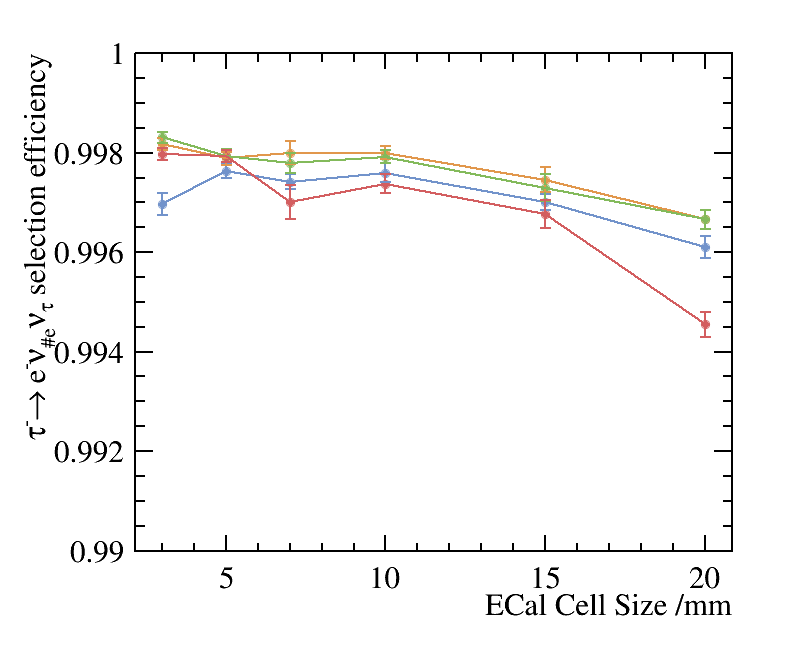
\includegraphics[width=.45\textwidth]{plots/decayMode0} 
%\qquad
%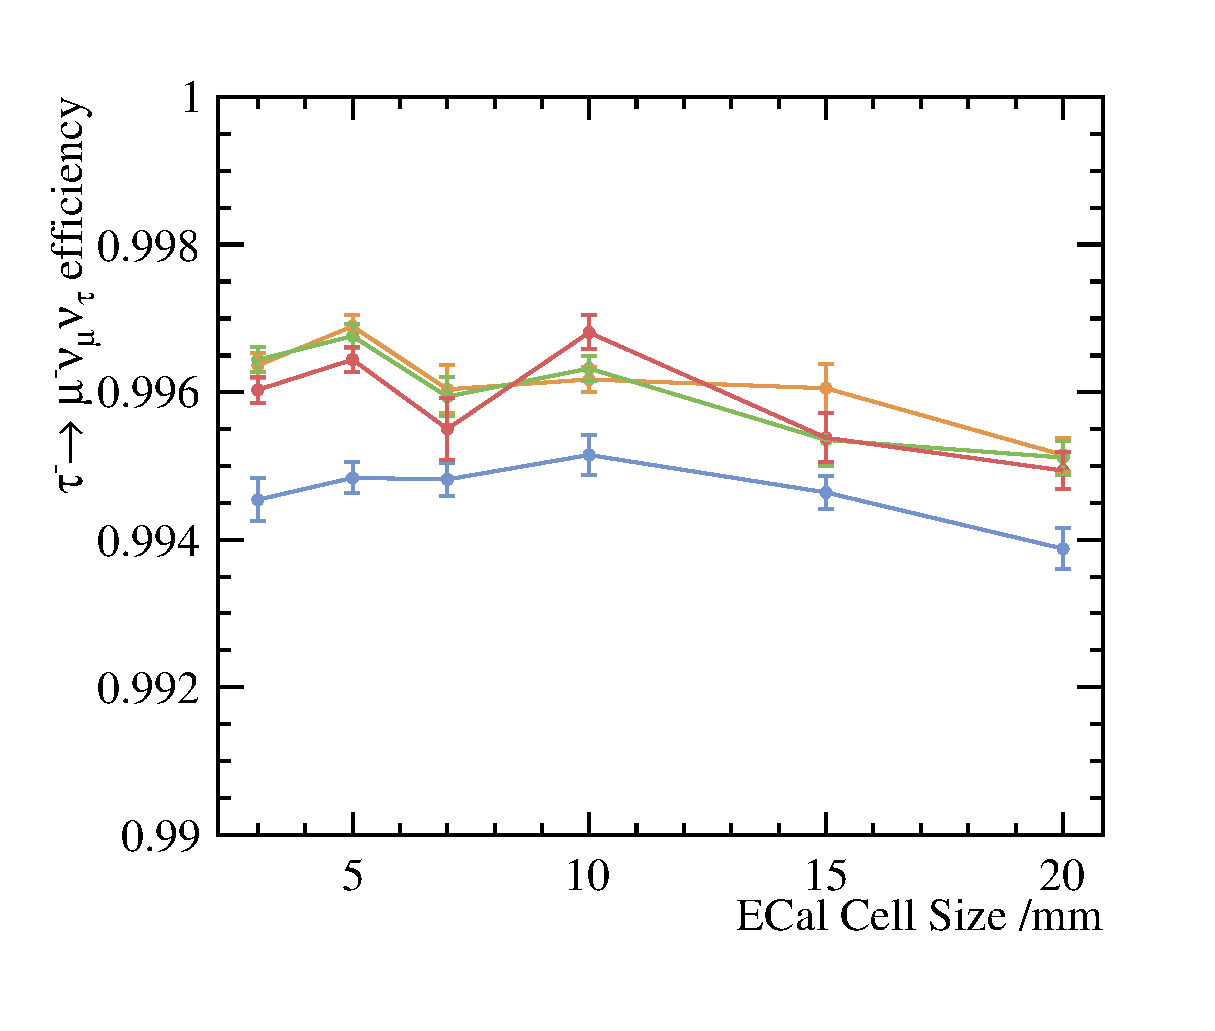
\includegraphics[width=.45\textwidth]{plots/decayMode1} 
%\qquad
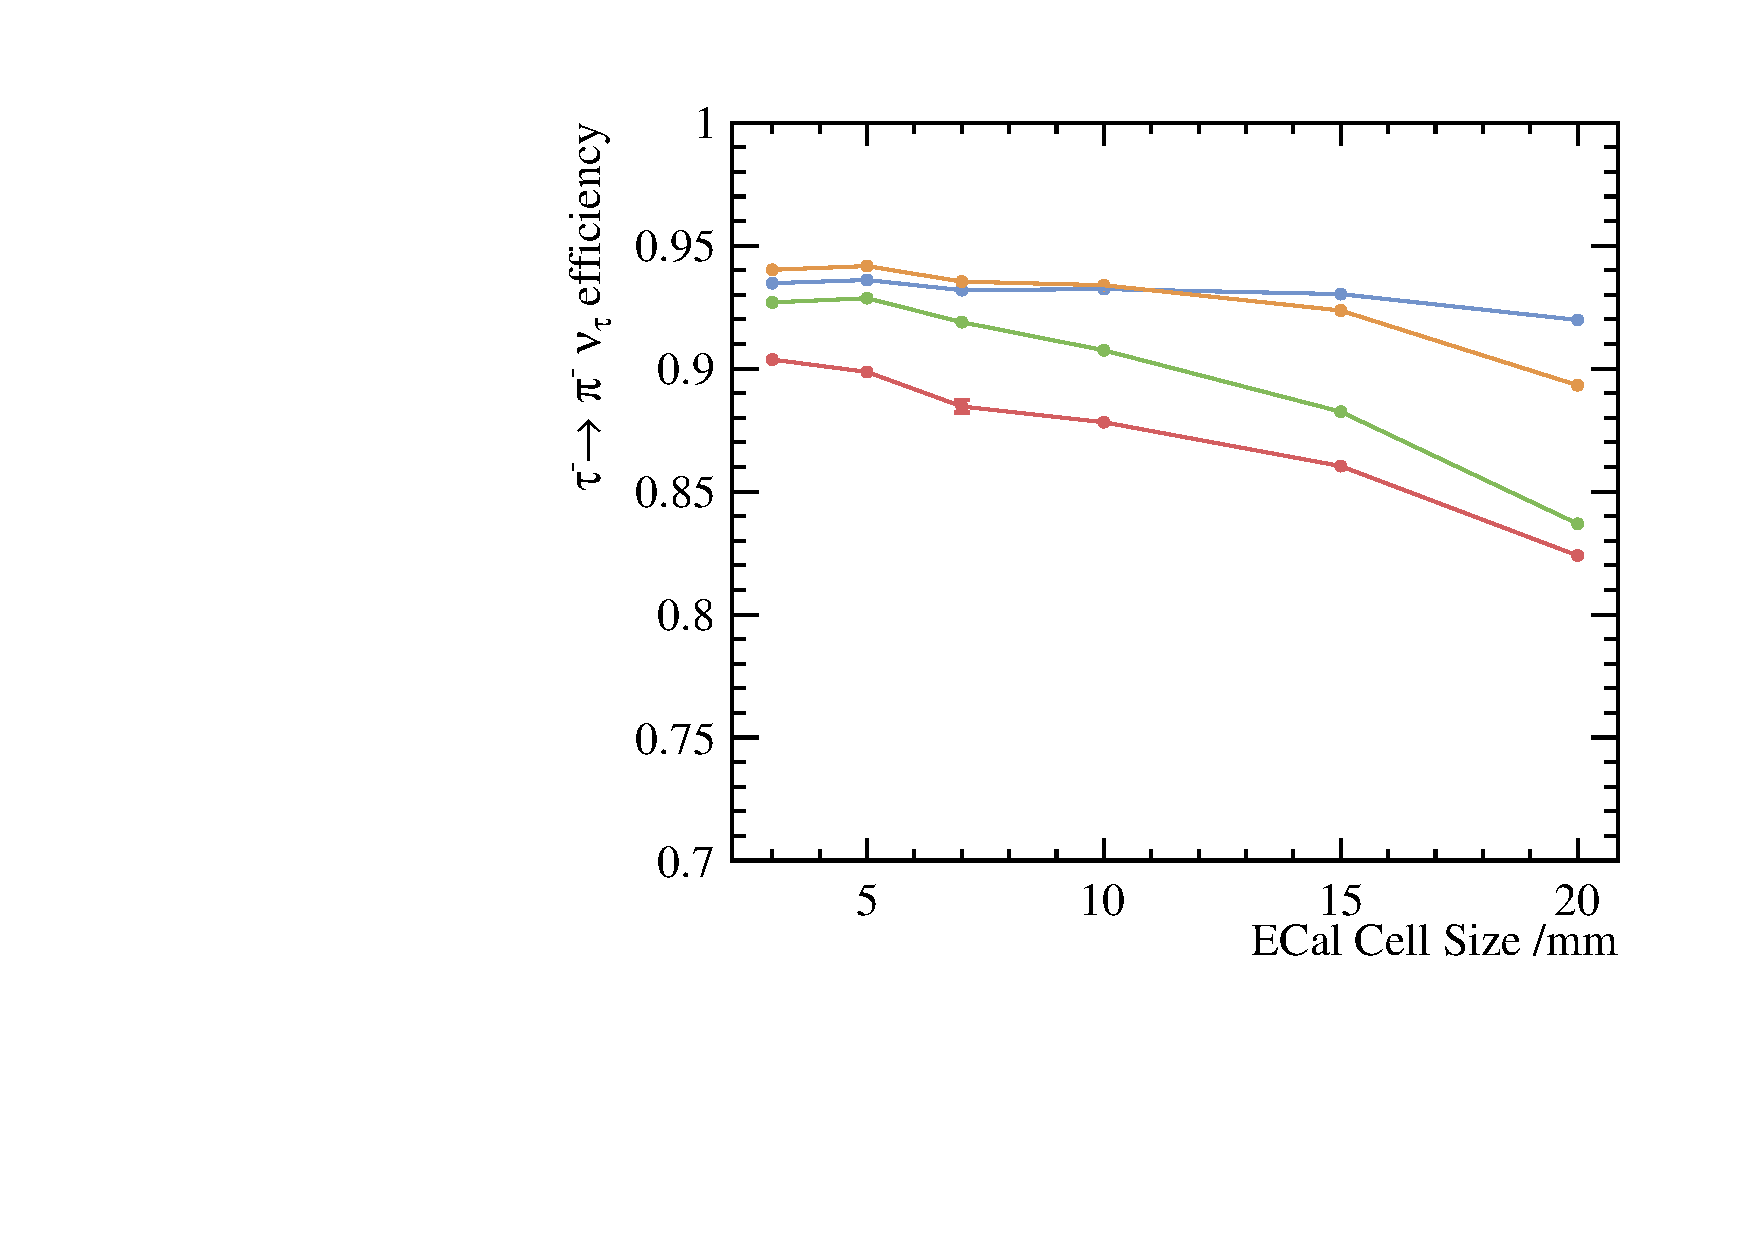
\includegraphics[width=.45\textwidth]{plots/decayMode2}
\qquad
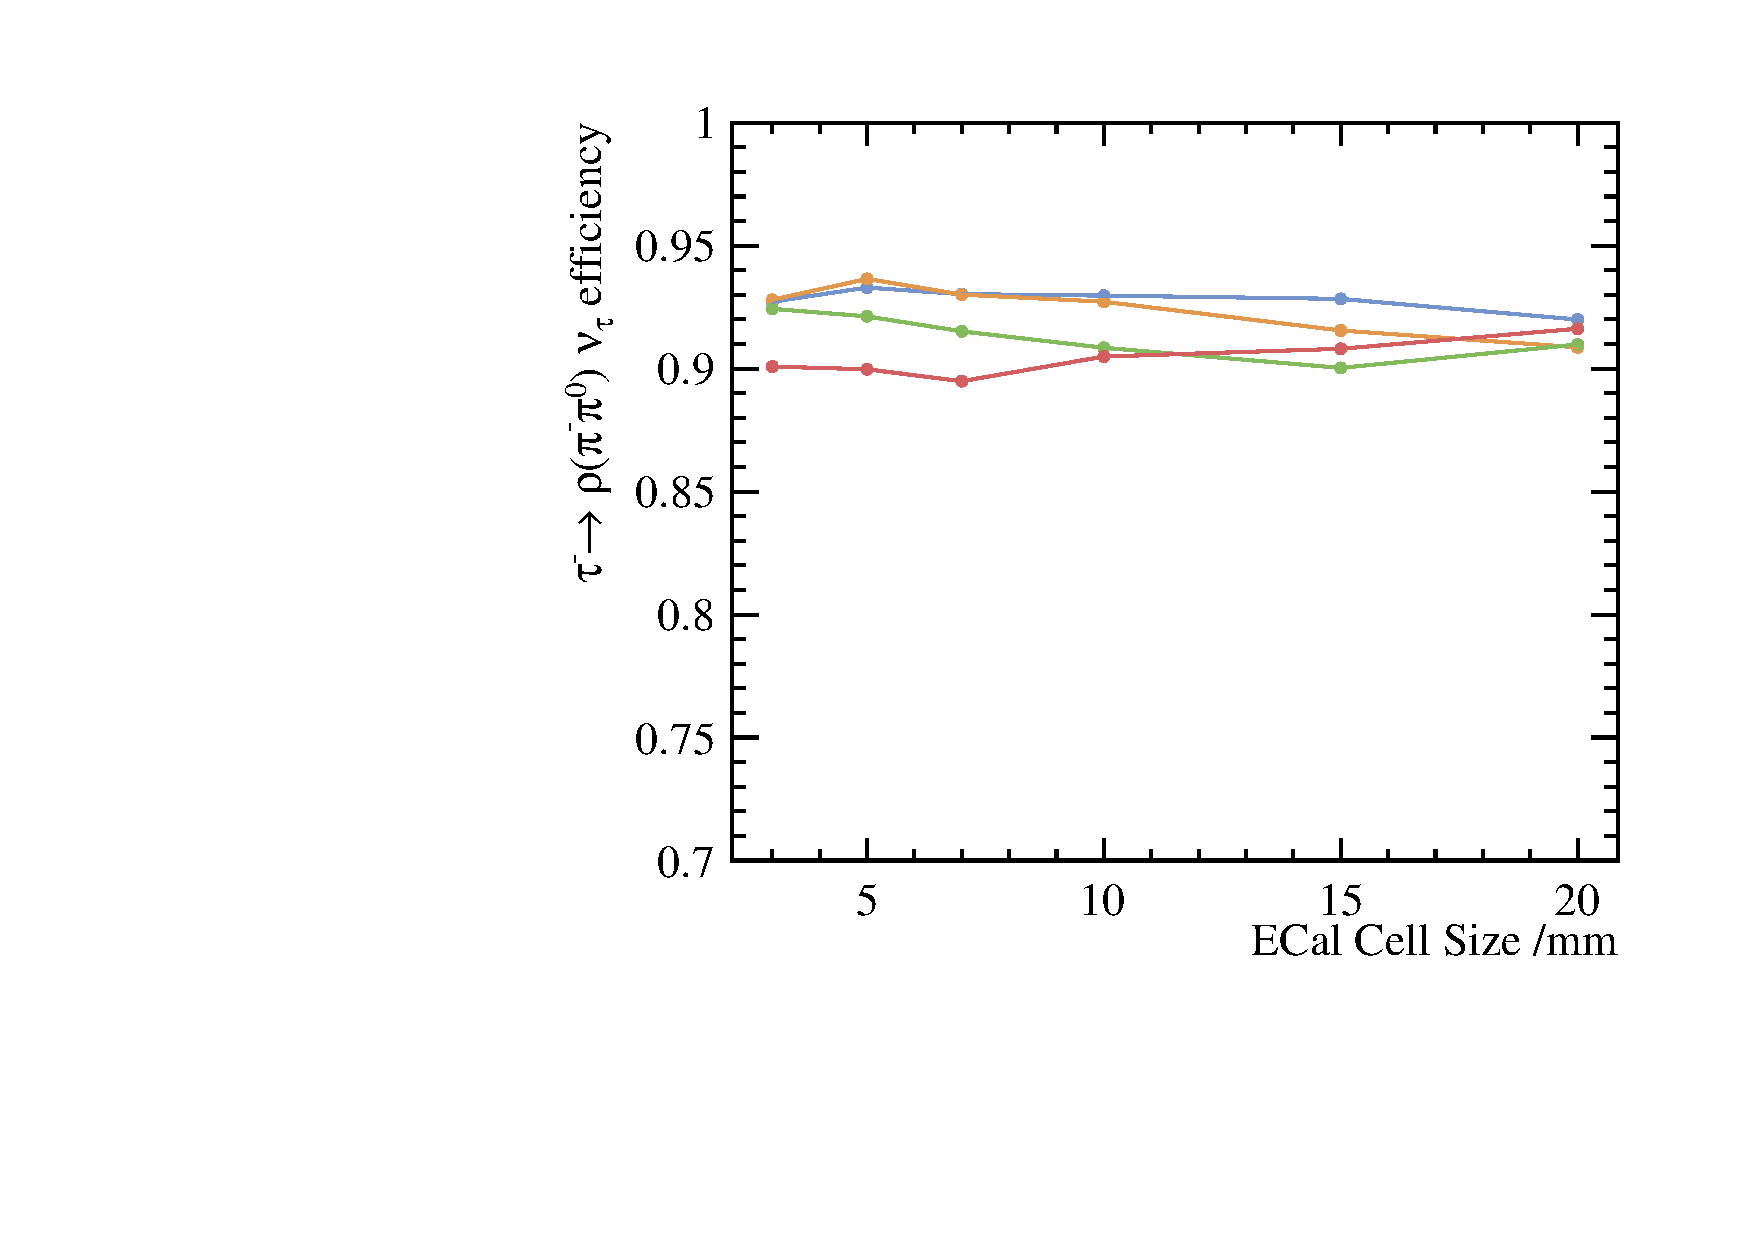
\includegraphics[width=.45\textwidth]{plots/decayMode3} 
\qquad
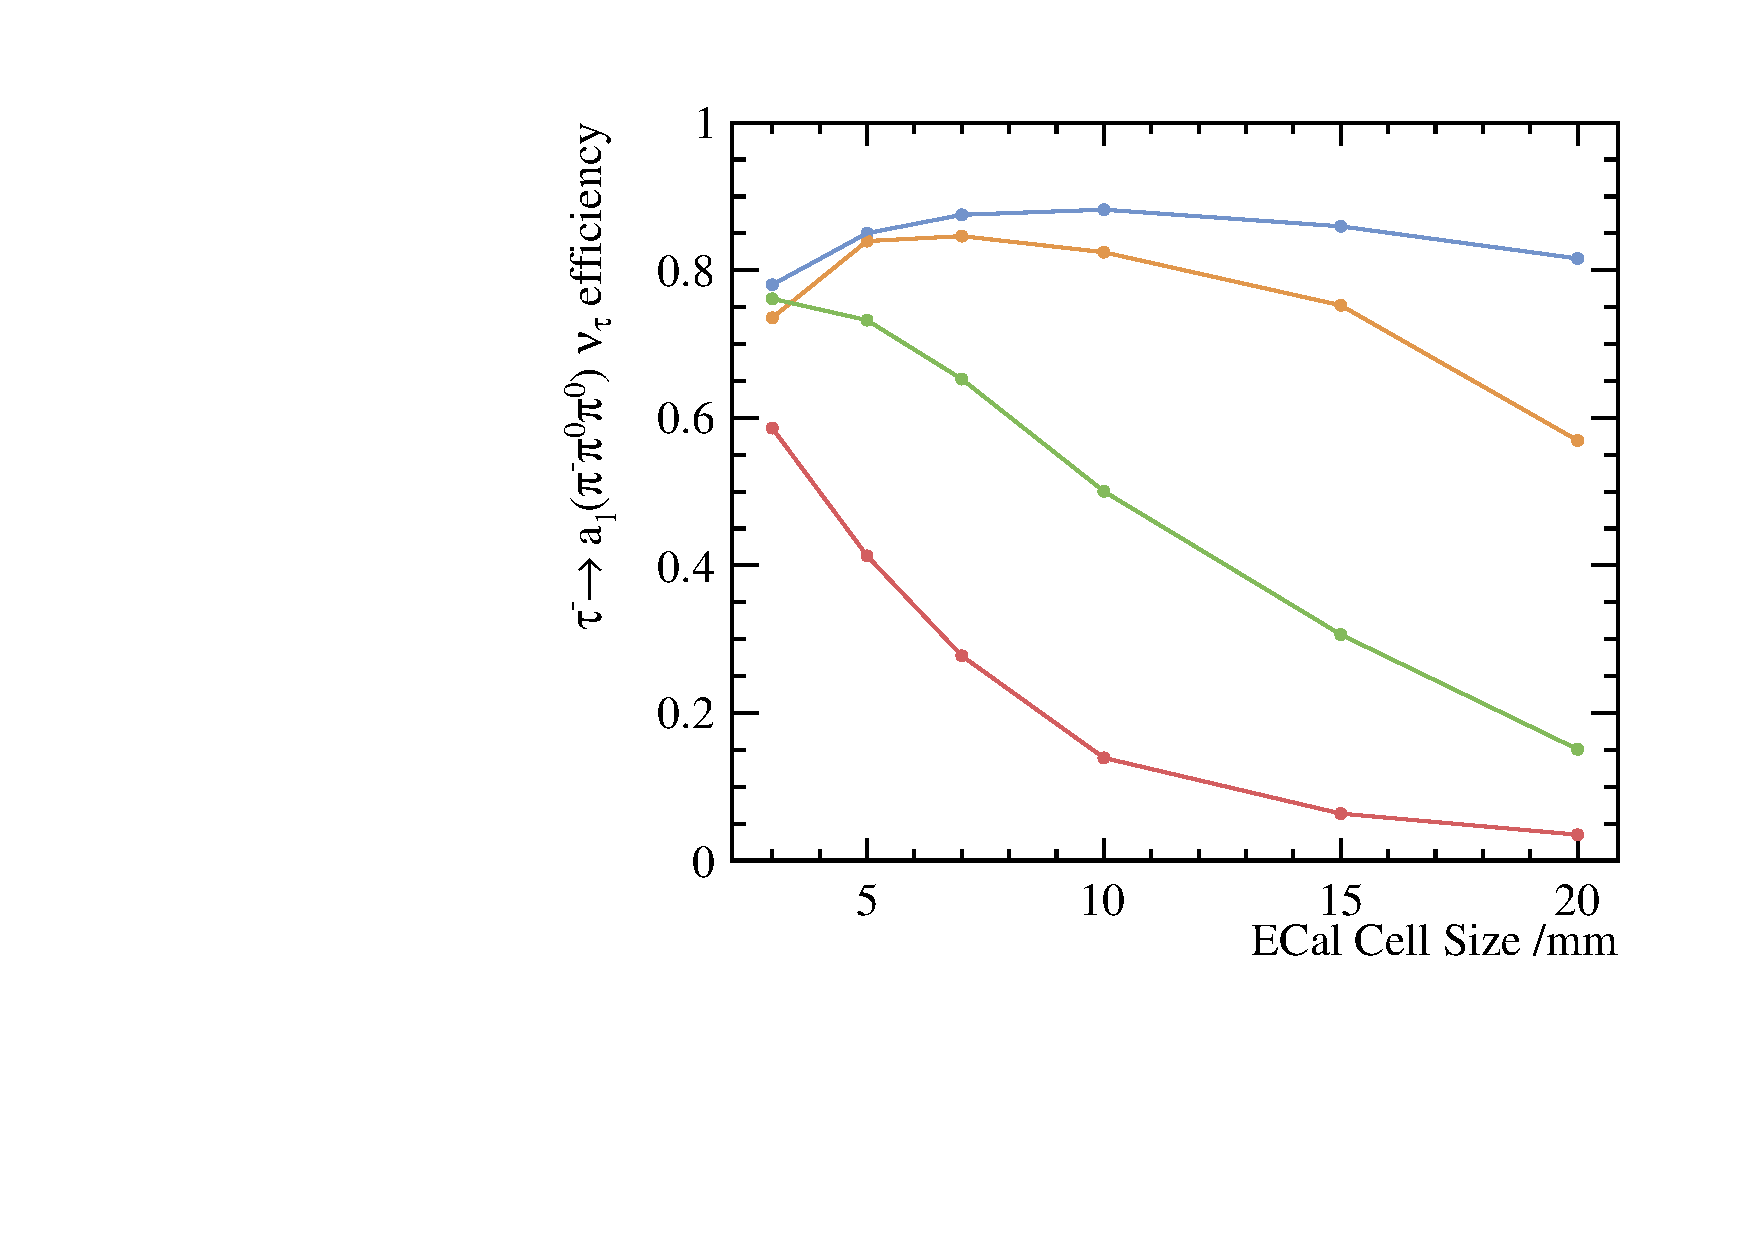
\includegraphics[width=.45\textwidth]{plots/decayMode4} 
\qquad
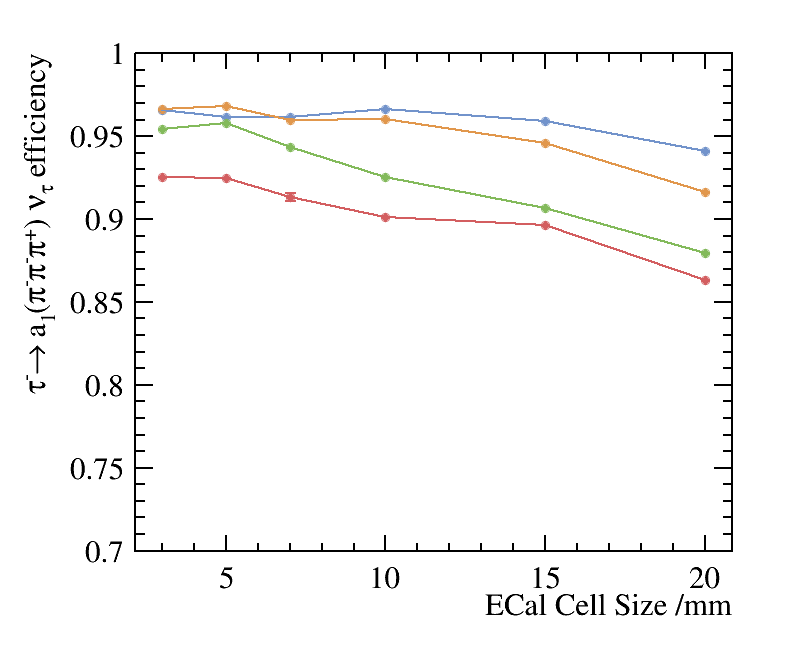
\includegraphics[width=.45\textwidth]{plots/decayMode5}
\qquad
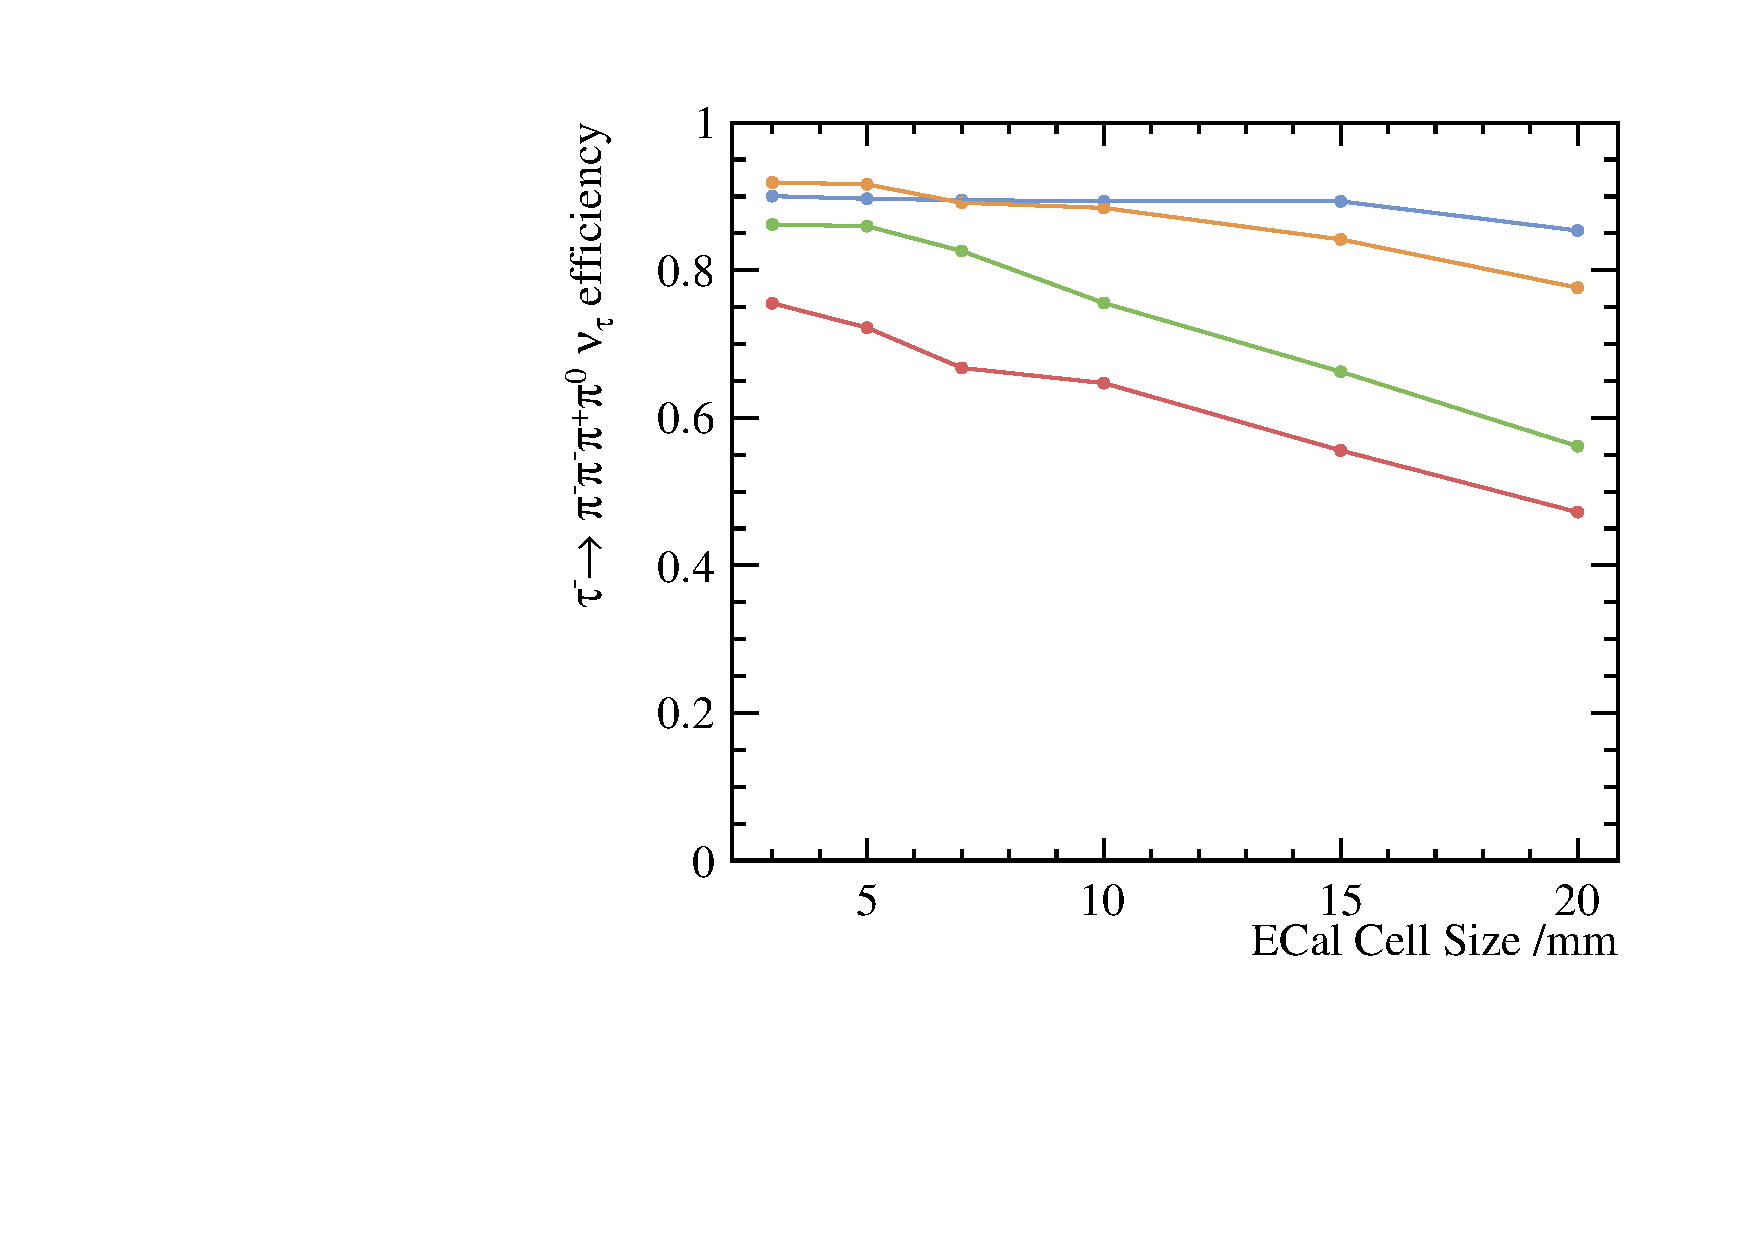
\includegraphics[width=.45\textwidth]{plots/decayMode6}
\qquad
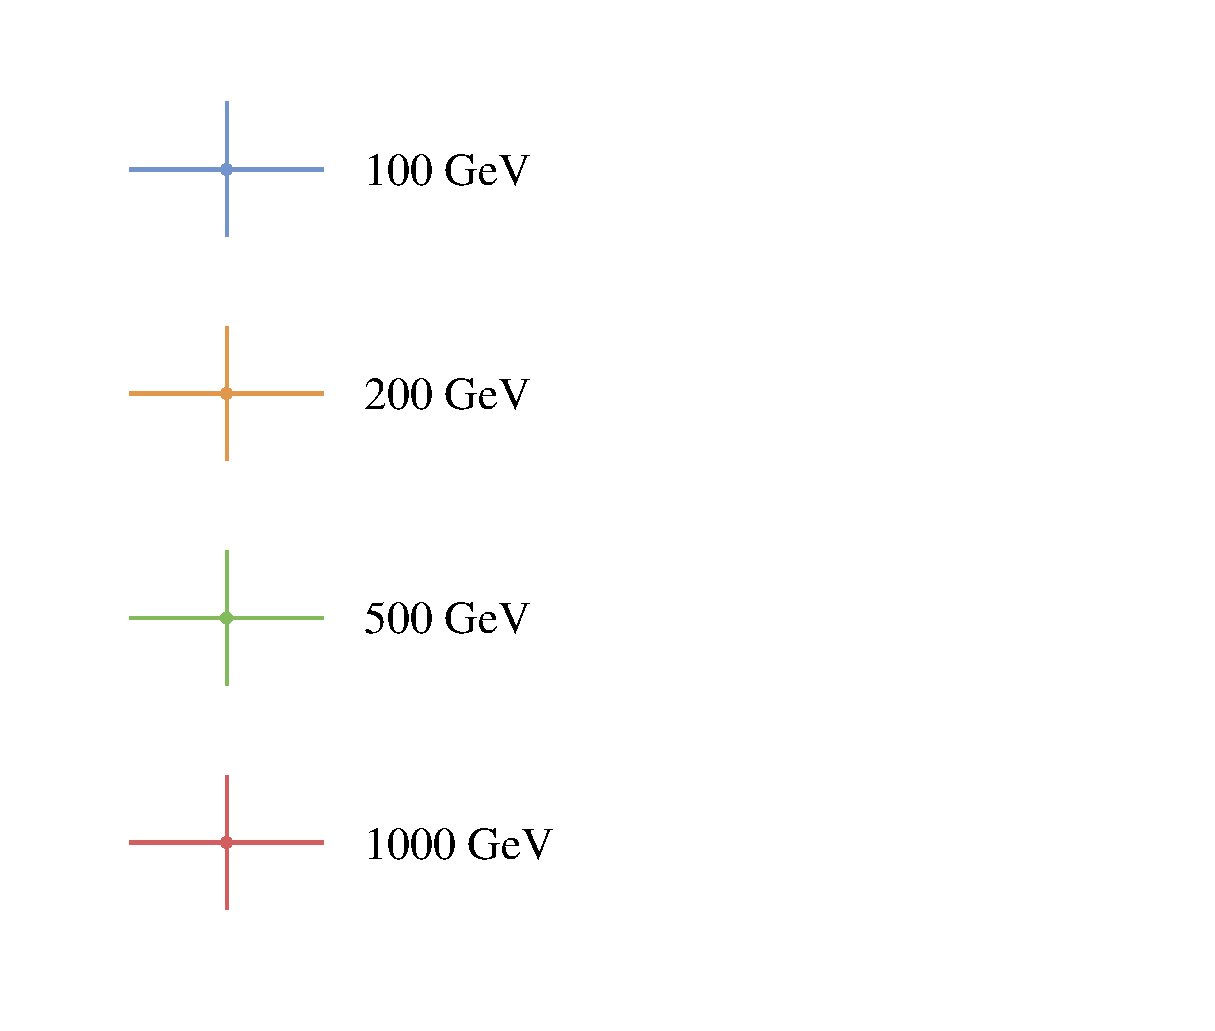
\includegraphics[width=.45\textwidth]{plots/legend}
%\qquad
%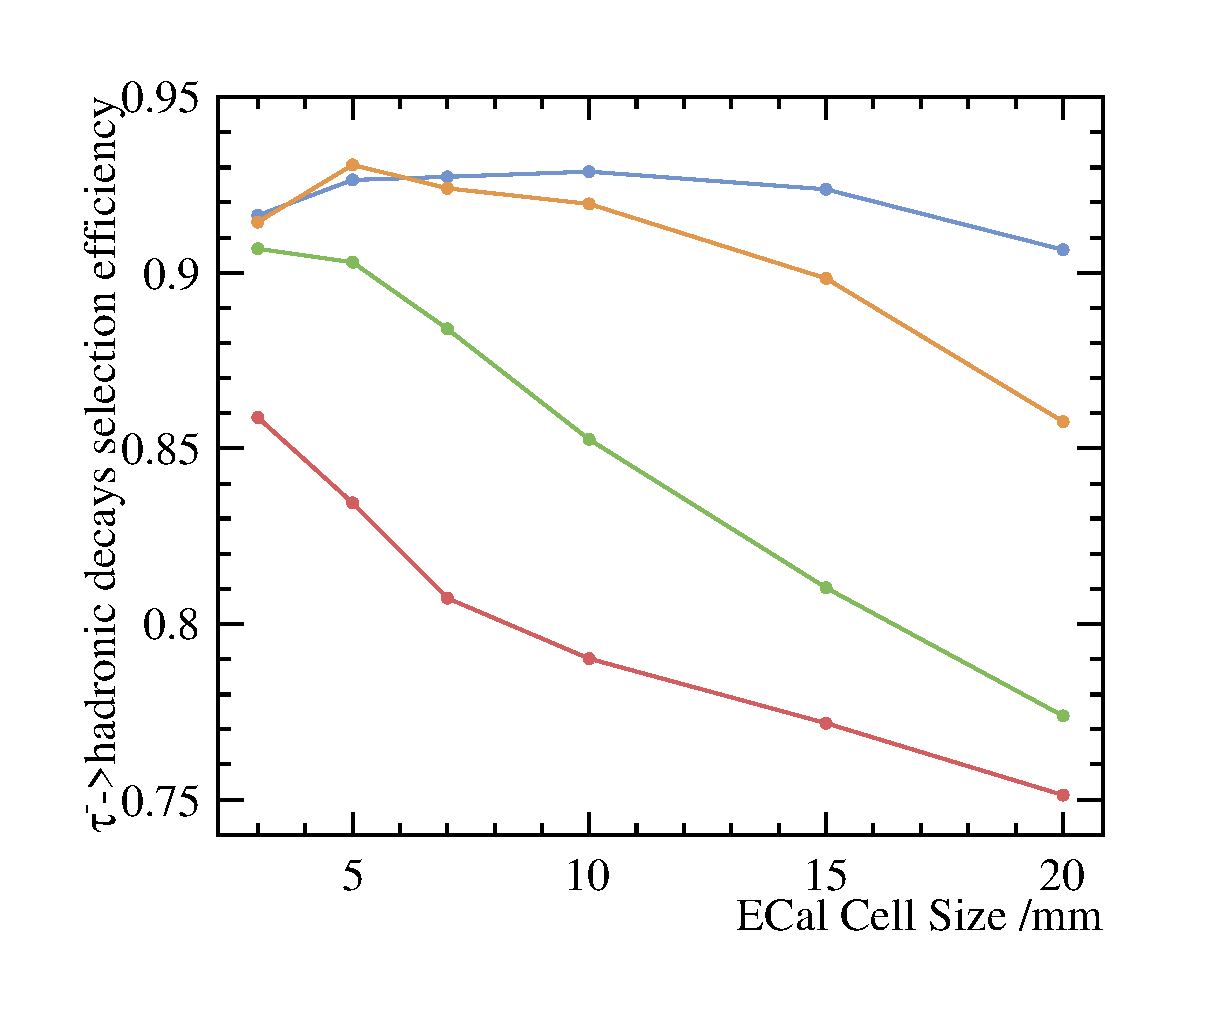
\includegraphics[width=.4\textwidth]{plots/hadEff}
% "\includegraphics" from the "graphicx" permits to crop (trim+clip)
% and rotate (angle) and image (and much more)
\caption{\label{fig:pion_efficiency} The selection efficiencies for various final states against the ECal cell size for different c.o.m. energies with the nominal CLIC\_ILD detector model are shown. The top left, top right, middle left, middle right and bottom left plots are for the \decayPion, \decayRho,  \decayAiPhoton, \decayAiPion  and \decayThreePionPhoton  final states respectively. From the top to the bottom, blue, orange, green and red lines are representing the \rootS = 100, 200, 500 and 1000\,GeV respectively. Note that the y axis are not the same for displaying purpose.}
\end{figure}

To compare the impact of the ECAL cell sizes and the \rootS energies on the separation of tau final states, the selection efficiencies were plotted in the figure~\ref{fig:pion_efficiency}. The leptonic decay selection efficiencies are not shown as they are similar across different ECal cell sizes. This is because the \Pepm and \PGmpm identifications mostly rely on the tracking system, which was not varied in this study. The energy deposited in the calorimeter are used for the association to the tracks but it has a small impact on the lepton identification. 

Overall, the hadronic decay selection efficiency decreases as the \rootS energy increases. This is due to the fact that when {\PGt}s are boosted at higher \rootS energies, the separation between decay products is smaller. Hence it is more difficult to reconstruct multi-photon final states correctly.

As the ECal cell sizes increase, the reconstruction efficiencies generally decrease. Larger cell sizes have lower spatial resolutions, making the separating of nearby photons more difficult.

For the \decayAiPhoton final state, the selection efficiency for 500\,GeV rises from ECal cell sizes 15\,mm to 20\,mm and the one for 1000\,GeV rises from 7\,, to 20\,mm actually goes up as cell size increases. This is because when the algorithm can not reconstruct four photons in the \decayAiPhoton final state, and the event topology would be very similar to the \decayRho final states. 

For the \rootS = 100 and 200\,GeV, the selection efficiency of the 5\,mm ECal cell size is better than that of the 3\,mm. One possible explanation is that the  and the PandoraPFA have been optimised for the nominal ILD detector with the 5\,mm ECal cell size, which shares the same ECal structure with the nominal CLIC\_ILD detector.

\begin{figure}[htbp]
\centering % \begin{center}/\end{center} takes some additional vertical space
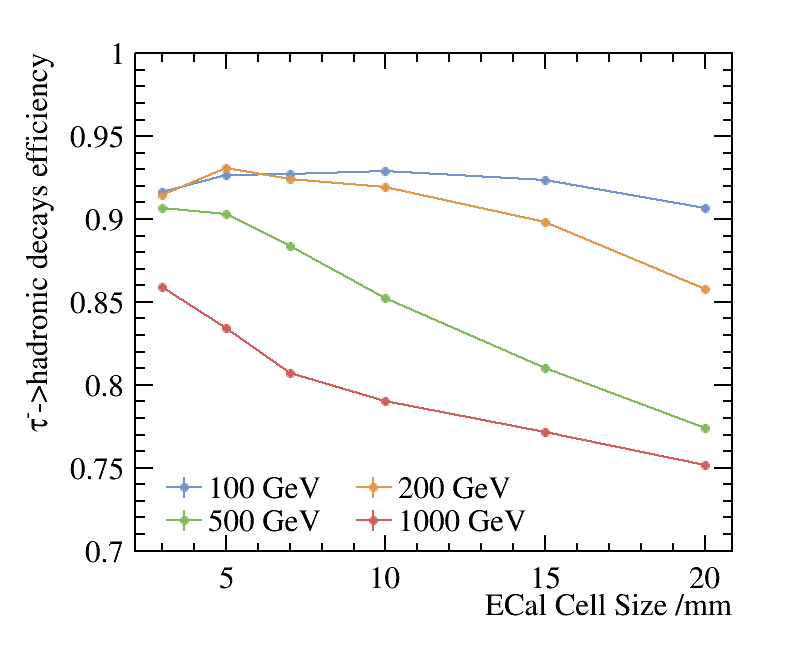
\includegraphics[width=.45\textwidth]{plots/hadronicEff}
% "\includegraphics" from the "graphicx" permits to crop (trim+clip)
% and rotate (angle) and image (and much more)
\caption{\label{fig:hadronic_efficiency} The \PGt hadronic decay selection efficiency against the ECal cell size for different \rootS energies with the nominal CLIC\_ILD detector model are shown. The blue, orange, green and red lines are representing the \rootS = 100, 200, 500 and 1000\,GeV respectively.}
\end{figure}

In order to compare the overall separation power of all the final states across c.o.m. energy and the ECal cell sizes, we constructed a single parameter function, the  \PGt hadronic decay final state efficiency function, 
\begin{equation}
\label{eq:had}
\varepsilon_{had} = \frac{\left(\Sigma_{i} {Br}_{i}\varepsilon_{i}\right)}{\Sigma_{i} {Br}_{i}}  \,,
\end{equation}
where $Br_{i}$ is the branching fraction of a hadronic final state after the generator level cut, $\varepsilon_{i}$ is the selection efficiency of the final state and the $i$ is summing over five hadronic decay final state of \PGt. Leptonic decays, \decayElectron and \decayMuon, were not included as the variation of the leptonic decay selection efficiency is small.

In the figure~\ref{fig:hadronic_efficiency}, \PGt hadronic decay final state efficiency, $\varepsilon_{had}$, against the ECal cell size with different \rootS is shown. $\varepsilon_{had}$ decreases when cell sizes increases and when \rootS increases.  Again, $\varepsilon_{had}$ of the 5\,mm ECal cell size is better than that of the 3\,mm for 100 and 200\,GeV lines possibly due the optimisation of the software fro the nominal ILD 5\,mm cell size.

The $\varepsilon_{had}$ is above 90\% for the ECal cell size from 3 to 20\,mm for the \rootS = 100\,GeV. For \rootS = 200\,GeV, the $\varepsilon_{had}$ decreases from over 90\% to 86\% for the ECal cell size from 3 to 20\,mm. The degradation of the $\varepsilon_{had}$ is significant for the 500 and 1000\,GeV lines, where the $\varepsilon_{had}$ drops from over 90\% to 77\%  and from 86\% to 75\% respectively. 

For low \rootS, namely 100 and 200\,GeV, up to 15\,mm cell sizes of ECal will give a good performance for \PGt hadronic decay modes separation, and the $\varepsilon_{had}$ is above 90\%. For the high c\rootS, namely 500 and 1000\,GeV, it is preferential to have a small ECal cell size for \PGt hadronic decay modes separation. There is about 15\% degradation of $\varepsilon_{had}$ for ECal cell size from 3 to 20\,mm.

%The degradation of $\varepsilon_{hadronic}$ is more significant for higher c.o.m. energy.

The paper illustrated the usage of reconstruction of the tau decay modes as a benchmark for the detector optimisation. 

%The high probability of correctly identifying the decay modes also showed the potential to measure the spin of the {\Ptau} with the CLIC machine.


%We discourage the use of inline figures (wrapfigure), as they may be
%difficult to position if the page layout changes.

%We suggest not to abbreviate: ``section'', ``appendix'', ``figure''
%and ``table'', but ``eq.'' and ``ref.'' are welcome. Also, please do
%not use \texttt{\textbackslash emph} or \texttt{\textbackslash it} for
%latin abbreviaitons: i.e., et al., e.g., vs., etc.



%\section{Sections}
%\subsection{And subsequent}
%\subsubsection{Sub-sections}
%\paragraph{Up to paragraphs.} We find that having more levels usually
%reduces the clarity of the article. Also, we strongly discourage the
%use of non-numbered sections (e.g.~\texttt{\textbackslash
%  subsubsection*}).  Please also see the use of
%``\texttt{\textbackslash texorpdfstring\{\}\{\}}'' to avoid warnings
%from the hyperref package when you have math in the section titles



\appendix
\section{Variables for multivariate analysis}

Here is a full list of all variables used in the multivariate analysis.

\begin{itemize}
\item  $\frac{E_{ECal,HCal}}{E_{tot}}$, charged:  Sum of energy deposited in ECal and HCal, divided by the energy of charged particles  
\item  $\frac{E_{ECal,HCal}}{E_{tot}}$, all:  	 Sum of energy deposited in ECal and HCal, divided by the energy of all particles  
\item  $m_{vis}$:     	 Invariant mass of visible particles in GeV   
\item  $\frac{E_{vis}}{E_{\PGtm}}$:	 Sum of energy of all particles, divided by the energy of \PGtm 
\item  $\frac{E_{charged}}{E_{\PGtm}}$:	 Sum of energy of charged particles, divided by the energy of \PGtm    
\item  $\frac{E_{\PGmm}}{E_{\PGtm}}$:	 Sum of energy of muons, divided by the energy of \PGtm    
\item  $\frac{E_{\Pem}}{E_{\PGtm}}$:	 Sum of energy of electrons, divided by the energy of \PGtm
\item  $\frac{E_{\PGg}}{E_{\PGtm}}$:	 Sum of energy of photons, divided by the energy of \PGtm  
\item  $\frac{E_{\PGpm}}{E_{\PGtm}}$:	 Sum of energy of charged pions, divided by the energy of \PGtm    
\item  $N_{charged}$:	 Number of charged particles    
\item  $N_{\PGmm}$:	 Number of muons    
\item  $N_{\Pem}$:	 Number of electrons
\item  $N_{\PGg}$:	 Number of photons  
\item  $N_{\PGpm}$:	 Number of charged pions    
\item  $m_{\PGg}$:     	 Invariant mass of photons in GeV   
\item  $m_{charged}$:     	 Invariant mass of charged particles in GeV   
\item  $m_{neutral}$:     	 Invariant mass of neutral particles in GeV   
\item  $m_{\PGpm}$:     	 Invariant mass of charged pions in GeV   
\item  $m_{\PGpz}, \PGrP{\PGpm\PGpz}$ hypothesis:     	 Fitted invariant mass of \PGpz for \PGrP{\PGpm\PGpz} hypothesis test  
\item  $m_{\PGrP{\PGpm\PGpz}}, \PGrP{\PGpm\PGpz}$ hypothesis:     	 Fitted invariant mass of \PGr for \PGrP{\PGpm\PGpz} hypothesis test  

\item  $m_{\PGpz1}, \PaDoP{\PGpm\PGpz\PGpz}$ hypothesis:     	 First fitted invariant mass of \PGpz, for \PaDoP{\PGpm\PGpz\PGpz} hypothesis test, ordered by closeness to the true \PGpz mass  
\item  $m_{\PGpz1}, \PaDoP{\PGpm\PGpz\PGpz}$ hypothesis:     	 Second fitted invariant mass of \PGpz, for \PaDoP{\PGpm\PGpz\PGpz} hypothesis test, ordered by closeness to the true \PGpz mass  
\item  $m_{\PaDoP{\PGpm\PGpz\PGpz}}, \PaDoP{\PGpm\PGpz\PGpz}$ hypothesis:     	 Second fitted invariant mass of \PaDoP{\PGpm\PGpz\PGpz}, for \PaDoP{\PGpm\PGpz\PGpz} hypothesis test 
\item  $\bar{E_{cell}}$:     	 Average energy deposited in a calorimeter cell in GeV 
\item  $d_{trans,shower}$:    Transverse shower width for electromagnetic shower profile, averaged for all clusters in the ECal 
\item  $l_{long,shower}$:    Longitudinal start layer for electromagnetic shower profile, averaged for all clusters in the ECal 
\item  $\Delta{l_{long,shower}}$:    Longitudinal discrepancy for electromagnetic shower profile, averaged for all clusters in the ECal 
\item  $\%MIP$:    Fraction of calorimeter hits registered as minimum ionised particles, averaged for all clusters in the ECal 
\item  $\frac{E}{P}$:   Energy divided by momentum, averaged for all clusters in the ECal 
\end{itemize}

\acknowledgments

The authors would like to thank P. G. Roloff for helping to generate the simulated samples. 

%\paragraph{Note added.} This is also a good position for notes added
%after the paper has been written.





% We suggest to always provide author, title and journal data:
% in short all the informations that clearly identify a document.

\bibliographystyle{h-physrev3}
\bibliography{bib}

%\begin{thebibliography}{99}

%\bibitem{a}
%Author, \emph{Title}, \emph{J. Abbrev.} {\bf vol} (year) pg.

%\bibitem{b}
%Author, \emph{Title},
%arxiv:1234.5678.

%\bibitem{c}
%Author, \emph{Title},
%Publisher (year).


% Please avoid comments such as "For a review'', "For some examples",
% "and references therein" or move them in the text. In general,
% please leave only references in the bibliography and move all
% accessory text in footnotes.

% Also, please have only one work for each \bibitem.


%\end{thebibliography}


\end{document}
